%\documentclass[hyperref={pdfpagelabels=false},slidetop,9pt]{beamer}
\documentclass[slidetop,8pt]{beamer}
\usepackage[T1]{fontenc}
\usepackage[utf8]{inputenc}
\newcommand{\id}{54}
\newcommand{\nom}{Liaisons mécaniques}
\newcommand{\sequence}{04}
\newcommand{\num}{01}
\newcommand{\type}{TP}
\newcommand{\descrip}{Modélisation d'un solide. Comportement des liaisons mécaniques. Modéliser les mécanismes du laboratoire par un schéma cinématique, paramétré.}
\newcommand{\competences}{A3-C4: Analyse d'architecture et de comportement \\ &  Mod1-C1: Isolement d'un solide ou d'un système de solides \\ &  Mod2-C10-1: Modèle de solide indéformable \\ &  Mod2-C11: Modélisation géométrique et cinématique des mouvements entre solides indéformables \\ &  Mod2-C12: Modélisation cinématique des liaisons entre solides \\ &  Mod2-C15: Modélisation des actions mécaniques \\ &  Rés-C6: Utilisation d'un solveur ou d'un logiciel multi physique \\ &  Com1-C1: Différents descripteurs introduits dans le programme \\ &  Com2-C4: Outils de communication}
\newcommand{\nbcomp}{9}
\newcommand{\systemes}{Plateforme Stewart}
\newcommand{\systemessansaccent}{Plateforme Stewart}
\newcommand{\ilot}{2}
\newcommand{\ilotstr}{02}
\newcommand{\dossierilot}{\detokenize{Ilot_02 Plateforme Stewart}}
\newcommand{\imageun}{Plateforme}

\newcommand{\urlsysteme}{\href{https://www.costadoat.fr/systeme/57}{Ressources système}}
\newcommand{\matlabsimscape}{\href{https://github.com/Costadoat/Sciences-Ingenieur/raw/master/Systemes/Plateforme Stewart/Plateforme_Stewart_Simscape.zip}{Modèle Simscape}}
\newcommand{\solidworks}{\href{https://github.com/Costadoat/Sciences-Ingenieur/raw/master/Systemes/Plateforme Stewart/Plateforme_Stewart_Solidworks.zip}{Modèle Solidworks}}
\newcommand{\edrawings}{\href{https://github.com/Costadoat/Sciences-Ingenieur/raw/master/Systemes/Plateforme Stewart/Plateforme_Stewart.EASM}{Modèle eDrawings}}
\newcommand{\test}{Stewart_param1}
\newcommand{\testi}{Stewart_param2}
\newcommand{\testii}{Stewart_param3}
\newcommand{\testiii}{Stewart_param4}
\newcommand{\testiiii}{Stewart_euler}
\usepackage{etex}
\usepackage{tikz}
\usepackage[european]{circuitikz}
\usepackage{pgf}
\usepackage[all]{xy}
\usepackage{pgfpages}
\usepackage{graphbox}
\usepackage{pdfpages}
\usepackage[adobe-utopia]{mathdesign}
\usepackage{ifthen}
\usepackage{cancel}
\usepackage{framed}
\usepackage{subfig}
\usepackage{tabularx}
\usepackage{setspace}
\usepackage{soul}
\usepackage{schemabloc}
\usepackage{eqnarray}
\usepackage[dot, phantomtext]{dashundergaps}
\usepackage{media9}
\usepackage{multimedia}
\usepackage{textcomp}

\author{Renaud Costadoat}
\institute{Lycée Dorian}

\usepackage{multido}
\usepackage{multirow}
\usepackage{multicol} % Portions de texte en colonnes
\usepackage{flafter}%floatants après la référence

\usepackage{color}
\usepackage{xcolor}
\usepackage{colortbl}

\usepackage[gen]{eurosym}
\usepackage{tikz}
%\usepackage{pstricks,pst-node,pst-tree,pst-solides3d}
\usepackage{lmodern}
\usepackage[francais]{babel}
\usepackage{pslatex}
\usetheme{renaud}
\usepackage{times}
\usepackage{amsmath}
\usepackage{verbatim}
\usepackage{moreverb}
%\usetikzlibrary{arrows,shapes}
\usepackage{graphicx}
\usepackage{psfrag}
\usepackage{wrapfig}
\usepackage{etoolbox}

\definecolor{gris25}{gray}{0.75}
\definecolor{bleu}{RGB}{18,33,98}
\definecolor{bleuf}{RGB}{42,94,171}
\definecolor{bleuc}{RGB}{231,239,247}
\definecolor{rougef}{RGB}{185,18,27}
\definecolor{rougec}{RGB}{255,188,204}%255,230,231
\definecolor{vertf}{RGB}{103,126,82}
\definecolor{vertc}{RGB}{220,255,191}

\setlength\parindent{24pt}
\parskip 7.2pt
\parindent 8pt

\newenvironment{rem}[1][\hsize]%
{%
    \def\FrameCommand
   {%
\rotatebox{90}{\textit{\textsf{Remarque}}} 
       {\color{bleuf}\vrule width 3pt}%
       \hspace{0pt}%must no space.
       \fboxsep=\FrameSep\colorbox{bleuc}%
  }%
    \MakeFramed{\hsize#1\advance\hsize-\width\FrameRestore}%
}%
{\endMakeFramed}%


\newenvironment{savoir}[1][\hsize]%
{%
    \def\FrameCommand
    {%
\rotatebox{90}{\textit{\textsf{Savoir}}} 
        {\color{bleuf}\vrule width 3pt}%
        \hspace{0pt}%must no space.
        \fboxsep=\FrameSep\colorbox{bleuc}%
    }%
    \MakeFramed{\hsize#1\advance\hsize-\width\FrameRestore}%
}%
{\endMakeFramed}%

\newenvironment{prob}[1][\hsize]%
{%
    \def\FrameCommand%
    {%
\rotatebox{90}{\textit{\textsf{Problematique}}} 
        {\color{rougef}\vrule width 3pt}%
        \hspace{0pt}%must no space.
        \fboxsep=\FrameSep\colorbox{rougec}%
    }%
    \MakeFramed{\hsize#1\advance\hsize-\width\FrameRestore}%
}%
{\endMakeFramed}%

\newenvironment{obj}[1][\hsize]%
{%
    \def\FrameCommand%
    {%
\rotatebox{90}{\textit{\textsf{Objectif}}} 
        {\color{vertf}\vrule width 3pt}%
        \hspace{0pt}%must no space.
        \fboxsep=\FrameSep\colorbox{vertc}%
    }%
    \MakeFramed{\hsize#1\advance\hsize-\width\FrameRestore}%
}%
{\endMakeFramed}%

\newenvironment{defi}[1][\hsize]%
{%
    \def\FrameCommand%
    {%
\rotatebox{90}{\textit{\textsf{Definition}}} 
        {\color{bleuf}\vrule width 3pt}%
        \hspace{0pt}%must no space.
        \fboxsep=\FrameSep\colorbox{rougec}%
    }%
    \MakeFramed{\hsize#1\advance\hsize-\width\FrameRestore}%
}%
{\endMakeFramed}%


\newenvironment{hypo}[1][\hsize]%
{%
    \def\FrameCommand%
    {%
\rotatebox{90}{\textit{\textsf{Hypothèse\\}}} 
        {\color{bleuf}\vrule width 3pt}%
        \hspace{0pt}%must no space.
        \fboxsep=\FrameSep\colorbox{bleuc}%
    }%
    \MakeFramed{\hsize#1\advance\hsize-\width\FrameRestore}%
}%
{\endMakeFramed}%


\newenvironment{prop}[1][\hsize]%
{%
    \def\FrameCommand%
    {%
\rotatebox{90}{\textit{\textsf{Propriété}}} 
        {\color{bleuf}\vrule width 3pt}%
        \hspace{0pt}%must no space.
        \fboxsep=\FrameSep\colorbox{bleuc}%
    }%
    \MakeFramed{\hsize#1\advance\hsize-\width\FrameRestore}%
}%
{\endMakeFramed}%

\newenvironment{props}[1][\hsize]%
{%
    \def\FrameCommand%
    {%
\rotatebox{90}{\textit{\textsf{Propriétés}}} 
        {\color{bleuf}\vrule width 3pt}%
        \hspace{0pt}%must no space.
        \fboxsep=\FrameSep\colorbox{bleuc}%
    }%
    \MakeFramed{\hsize#1\advance\hsize-\width\FrameRestore}%
}%
{\endMakeFramed}%

\newenvironment{exemple}[1][\hsize]%
{%
    \def\FrameCommand%
    {%
\rotatebox{90}{\textit{\textsf{Exemple}}} 
        {\color{vertf}\vrule width 3pt}%
        \hspace{0pt}%must no space.
        \fboxsep=\FrameSep\colorbox{vertc}%
    }%
    \MakeFramed{\hsize#1\advance\hsize-\width\FrameRestore}%
}%
{\endMakeFramed}%

\newenvironment{resultat}[1][\hsize]%
{%
    \def\FrameCommand%
    {%
\rotatebox{90}{\textit{\textsf{Résultat}}} 
        {\color{rougef}\vrule width 3pt}%
%        {\color{bleuf}\vrule width 3pt}%
        \hspace{0pt}%must no space.
        \fboxsep=\FrameSep\colorbox{rougec}%
    }%
    \MakeFramed{\hsize#1\advance\hsize-\width\FrameRestore}%
}%
{\endMakeFramed}%

\newenvironment{methode}[1][\hsize]%
{%
    \def\FrameCommand%
    {%
\rotatebox{90}{\textit{\textsf{Méthode\\}}} 
        {\color{rougef}\vrule width 3pt}%
        \hspace{0pt}%must no space.
        \fboxsep=\FrameSep\colorbox{rougec}%
    }%
    \MakeFramed{\hsize#1\advance\hsize-\width\FrameRestore}%
}%
{\endMakeFramed}%

\newenvironment{theo}[1][\hsize]%
{%
    \def\FrameCommand%
    {%
\rotatebox{90}{\textit{\textsf{Théorème\\}}} 
        {\color{rougef}\vrule width 3pt}%
        \hspace{0pt}%must no space.
        \fboxsep=\FrameSep\colorbox{rougec}%
    }%
    \MakeFramed{\hsize#1\advance\hsize-\width\FrameRestore}%
}%
{\endMakeFramed}%

\newenvironment{warn}[1][\hsize]%
{%
    \def\FrameCommand%
    {%
\rotatebox{90}{\textit{\textsf{Attention\\}}} 
        {\color{rougef}\vrule width 3pt}%
        \hspace{0pt}%must no space.
        \fboxsep=\FrameSep\colorbox{rougec}%
    }%
    \MakeFramed{\hsize#1\advance\hsize-\width\FrameRestore}%
}%
{\endMakeFramed}%

% \usepackage{pstricks}
%\usepackage{minitoc}
% \setcounter{minitocdepth}{4}

\setcounter{tocdepth}{2}

% \mtcselectlanguage{french} 

%\usepackage{draftcopy}% "Brouillon"
% \usepackage{floatflt}
\usepackage{psfrag}
%\usepackage{listings} % Permet d'insérer du code de programmation
\renewcommand{\baselinestretch}{1.2}

% Changer la num�rotation des figures :
% ------------------------------------
% \makeatletter
% \renewcommand{\thefigure}{\ifnum \c@section>\z@ \thesection.\fi
%  \@arabic\c@figure}
% \@addtoreset{figure}{section}
% \makeatother
 


%%%%%%%%%%%%
% Définition des vecteurs %
%%%%%%%%%%%%
 \newcommand{\vect}[1]{\overrightarrow{#1}}

%%%%%%%%%%%%
% Définition des torseusr %
%%%%%%%%%%%%

 \newcommand{\torseur}[1]{%
\left\{{#1}\right\}
}

\newcommand{\torseurcin}[3]{%
\left\{\mathcal{#1} \left(#2/#3 \right) \right\}
}

\newcommand{\torseurstat}[3]{%
\left\{\mathcal{#1} \left(#2\rightarrow #3 \right) \right\}
}

 \newcommand{\torseurc}[8]{%
%\left\{#1 \right\}=
\left\{
{#1}
\right\}
 = 
\left\{%
\begin{array}{cc}%
{#2} & {#5}\\%
{#3} & {#6}\\%
{#4} & {#7}\\%
\end{array}%
\right\}_{#8}%
}

 \newcommand{\torseurcol}[7]{
\left\{%
\begin{array}{cc}%
{#1} & {#4}\\%
{#2} & {#5}\\%
{#3} & {#6}\\%
\end{array}%
\right\}_{#7}%
}

 \newcommand{\torseurl}[3]{%
%\left\{\mathcal{#1}\right\}_{#2}=%
\left\{%
\begin{array}{l}%
{#1} \\%
{#2} %
\end{array}%
\right\}_{#3}%
}

 \newcommand{\vectv}[3]{%
\vect{V\left( {#1} \in {#2}/{#3}\right)}
}


\newcommand{\vectf}[2]{%
\vect{R\left( {#1} \rightarrow {#2}\right)}
}

\newcommand{\vectm}[3]{%
\vect{\mathcal{M}\left( {#1}, {#2} \rightarrow {#3}\right)}
}


 \newcommand{\vectg}[3]{%
\vect{\Gamma \left( {#1} \in {#2}/{#3}\right)}
}

 \newcommand{\vecto}[2]{%
\vect{\Omega\left( {#1}/{#2}\right)}
}

\newcommand{\reponse}[1][4]
{
\multido{}{#1}
{
\begin{center}
\makebox[0.9\linewidth]{\dotfill} \end{center}
}}


% }$$\left\{\mathcal{#1} \right\}_{#2} =%
% \left\{%
% \begin{array}{c}%
%  #3 \\%
%  #4 %
% \end{array}%
% \right\}_{#5}}


%  ------------------------------------------
% | Modification du formatage des sections : | 
%  ------------------------------------------

% Grands titres :
% ---------------

\newcommand{\titre}[1]{%
\begin{center}
      \bigskip
      \rule{\textwidth}{1pt}
      \par\vspace{0.1cm}
      
      \textbf{\large #1}
      \par\rule{\textwidth}{1pt}
    \end{center}
    \bigskip
  }

% Supprime le numéro du chapitre dans la numérotation des sections:
% -----------------------------------------------------------------
\makeatletter
\renewcommand{\thesection}{\@arabic\c@section}
\makeatother


% \titleformat{\chapter}[display]
% {\normalfont\Large\filcenter}
% {}
% {1pc}
% {\titlerule[1pt]
%   \vspace{1pc}%
%   \Huge}[\vspace{1ex}%
% \titlerule]


%%%% Chapitres Comme PY Pechard %%%%%%%%%
% numéro du chapitre
\DeclareFixedFont{\chapnumfont}{OT1}{phv}{b}{n}{80pt}
% pour le mot " Chapitre "
\DeclareFixedFont{\chapchapfont}{OT1}{phv}{m}{it}{40pt}
% pour le titre
\DeclareFixedFont{\chaptitfont}{T1}{phv}{b}{n}{25pt}

\definecolor{gris}{gray}{0.75}
\setbeamertemplate{section in toc}[sections numbered]

\newlength{\RoundedBoxWidth}
\newsavebox{\GrayRoundedBox}
\newenvironment{GrayBox}[1][\dimexpr\textwidth-4.5ex]%
   {\setlength{\RoundedBoxWidth}{\dimexpr#1}
    \begin{lrbox}{\GrayRoundedBox}
       \begin{minipage}{\RoundedBoxWidth}}%
   {   \end{minipage}
    \end{lrbox}
    \begin{center}
    \begin{tikzpicture}%
       \draw node[draw=bleuf,fill=bleuc,rounded corners,%
             inner sep=2ex,text width=\RoundedBoxWidth]%
             {\usebox{\GrayRoundedBox}};
    \end{tikzpicture}
    \end{center}}
    
\ifdef{\prive}{\pgfpagesuselayout{2 on 1}[a4paper,border shrink=0mm]}
\ifdef{\prive}{\setbeamertemplate{navigation symbols}{}}
\setbeamertemplate{itemize item}[ball]
%\setbeamertemplate{blocks}[rounded]%[shadow=true]
\setbeamercolor{block title}{fg=white,bg=grisf}        % titre block normal 
\setbeamercolor{block body}{fg=grisf,bg=grisc!50}      % corps block normal
\setbeamercolor{block body alerted}{fg=white,bg=warning}   % idem pour un block alerte

\title{\nom}
\date{S\sequence \ - \type\num}

\begin{document}
\shorthandoff{:!}
\bibliographystyle{abbrvnat-fr}

\usebackgroundtemplate%
{%
    \centering
\includegraphics[width=\paperwidth]{../../img/fond2}%
}

{
\setbeamertemplate{navigation symbols}{}
\setbeamertemplate{headline}[pagetitre]
\setbeamertemplate{footline}[pagetitre]
\usebackgroundtemplate{\centering
\includegraphics[width=\paperwidth]{../../img/fond}}
\frame{\titlepage}
}



\section{Introduction}

{\frame{
\frametitle{Théorie des mécanismes}

\begin{savoir}

Vous devez être capables de modéliser le contact entre deux pièces (ou classes d'équivalences) par une liaison.

\begin{itemize}
 \item Quelles sont les types de liaison,
 \item Comment paramétrer une liaison,
 \item Comment représenter une liaison.
\end{itemize}
\end{savoir}

\begin{prob}
La liaison entre deux classes d'équivalence peut avoir ses mobilités contraintes par plus d'une liaison élémentaire.
\begin{itemize}
 \item \textit{Problème: Comment trouver les mobilités de la liaison globale à partir des mobilités des liaisons élémentaires ?}
 \item \textbf{Perspectives}: Savoir trouver la liaison globale entre deux classes d'équivalence.
\end{itemize}
\end{prob}
}}

{\frame{
\frametitle{Liaisons équivalentes}

\begin{itemize}
 \item Les liaisons équivalentes sont constituées à partir d'un groupe de liaisons élémentaires.
 \item Elles apparaissent entre deux solides dont les mouvements relatifs sont déterminés par au moins deux liaisons.
 \item Ainsi, les mobilités de la liaison globale sont déterminées grâce à la combinaison de ces liaisons élémentaires.
\end{itemize}

\vfill

\begin{exemple}
\begin{minipage}{0.48\linewidth}
Ex: La liaison globale entre une table et le sol constituée de 4 liaisons ponctuelles et une liaison appui plan. Vrai si le nombre de pieds est supérieur ou égal à 3.
\end{minipage}
\hfill
\begin{minipage}{0.47\linewidth}
\centering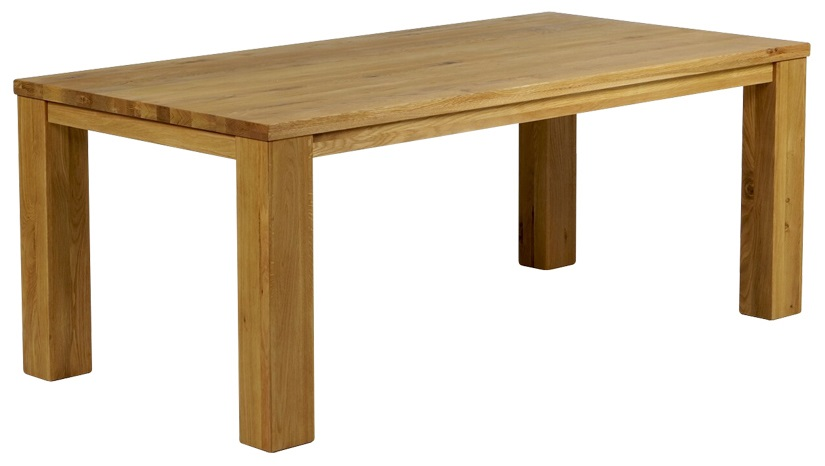
\includegraphics[width=0.7\linewidth]{img/table}
\end{minipage}
\end{exemple}
}}

{\frame{
\frametitle{Méthode d'étude des mécanismes}

\begin{rem}
 \begin{itemize}
  \item L'étude d'un mécanisme ne peut s'effectuer qu'après avoir réussi sa modélisation. 
  \item Afin de le modéliser il faut avoir compris le fonctionnement d'un mécanisme, ce qui n'est pas simple surtout si ce dernier est complexe (beaucoup de pièces...)
  \item L'utilisation de la méthode suivante permet de simplifier cette étude.
 \end{itemize}
\end{rem}

\begin{enumerate}
\item À partir du dessin d'ensemble ou du système réel, regrouper les pièces liées par des liaisons encastrement (liaisons à mobilité nulle).
\item En examinant les surfaces de contact, et \textit{en enlevant les éléments intermédiaires} comme les roulements, les ressorts,... définir les liaisons entre ces solides, \textit{deux à deux}, en déterminant les \textbf{mouvements relatifs possibles}.
\item \textbf{Numéroter} les solides en attribuant conventionnellement le numéro 0 au bâti ou au solide de référence.	
\end{enumerate}
}}

{\frame{
\frametitle{Modélisation d'un mécanisme, méthode d'analyse}

\begin{itemize}
 \item Un mécanisme étant un ensemble de \textbf{solides et de liaisons organisé}, il est indispensable d'en faire une \textbf{analyse} et une \textbf{représentation} logique, conforme à sa représentation.
 \vfill
 \item Outils appropriés disponibles par type d'étude:
  \begin{itemize}
	 \item Étude \textbf{géométrique} et/ou \textbf{cinématique}: \textit{Le graphe de structure (ou des liaisons) et le schéma cinématique}
	\begin{itemize}
 		\item Les solides sont les \textbf{classes d'équivalence} (pièces liées par encastrement)
 		\item Les liaisons représentées sont des \textbf{liaisons globales} (1 liaison entre 2 solides)
	\end{itemize}
	 \item Étude des efforts dans les liaisons, en \textbf{statique} ou \textbf{dynamique}: \textit{Le graphe des contacts et le schéma d'architecture}
	\begin{itemize}
 		\item Les solides sont les \textbf{classes d'équivalence},
 		\item Les liaisons représentées sont des \textbf{liaisons élémentaires} (1 ou plusieurs liaison(s) entre 2 solides)
  	\end{itemize}
  \end{itemize}
\end{itemize}
}}

{\frame{
\frametitle{Graphes associés au mécanisme}

Le \textbf{graphe associé au mécanisme} est construit en associant à chacun des solides un sommet et à chacune des liaisons mécaniques un arc matérialisé par un segment de droite. Les sommets sont numérotés en correspondance avec le schéma cinématique.

\hfill

\begin{center}
 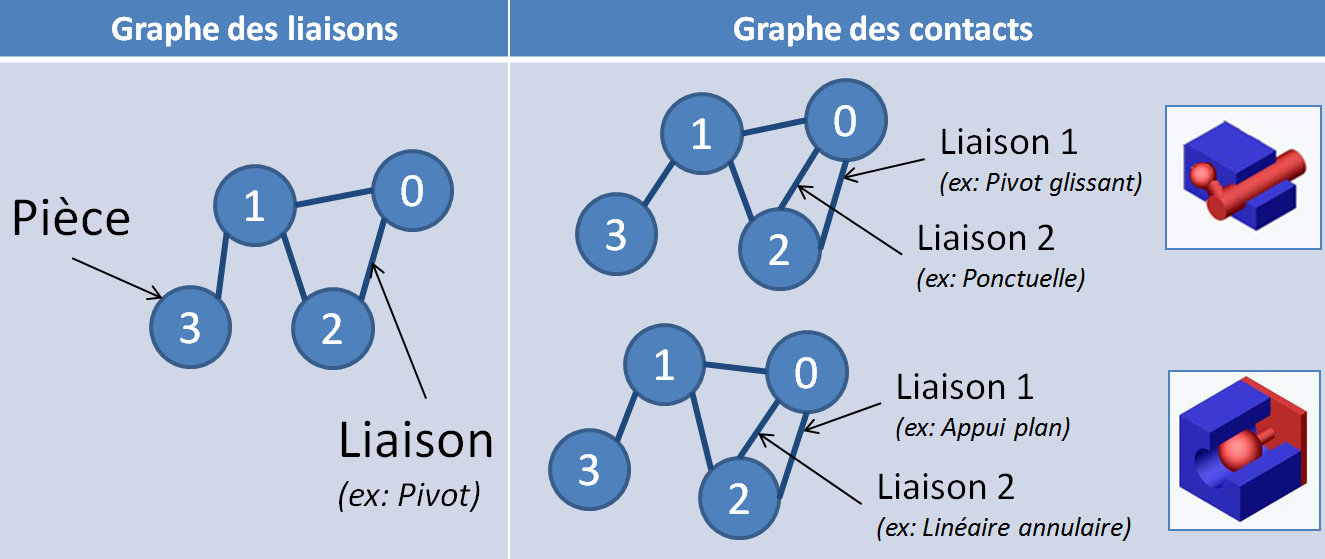
\includegraphics[width=0.8\linewidth]{img/graphe}
\end{center}
}}

{\frame{
\frametitle{Chaîne fermée simple ou cycle}

\begin{itemize}
 \item Un cycle est un chemin du graphe qui part d'un sommet et y revient sans passer plus d'une fois par un sommet
 \item $\gamma$ est le nombre de boucles indépendantes d'un graphe
\end{itemize}

\vfill

\begin{minipage}{0.48\linewidth}
 \centering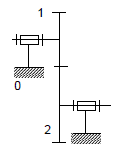
\includegraphics[width=0.6\linewidth]{img/graphe1}
\end{minipage}
\hfill
\begin{minipage}{0.48\linewidth}
\ifdef{\public}{\centering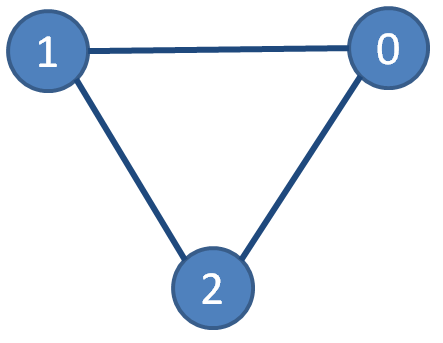
\includegraphics[width=0.6\linewidth]{img/graphe1_1}}{}
\end{minipage}
}}

{\frame{
\frametitle{Chaîne ouverte}

\begin{itemize}
 \item Un mécanisme est dit à chaîne ouverte s'il n'existe pas de cycle. En partant du bâti, on va de solide en solide vers un solide terminal.
\end{itemize}

\vfill

\begin{minipage}{0.48\linewidth}
 \centering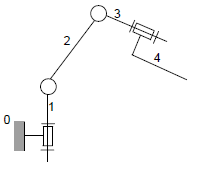
\includegraphics[width=0.8\linewidth]{img/graphe2}
\end{minipage}
\hfill
\begin{minipage}{0.48\linewidth}
\ifdef{\public}{\centering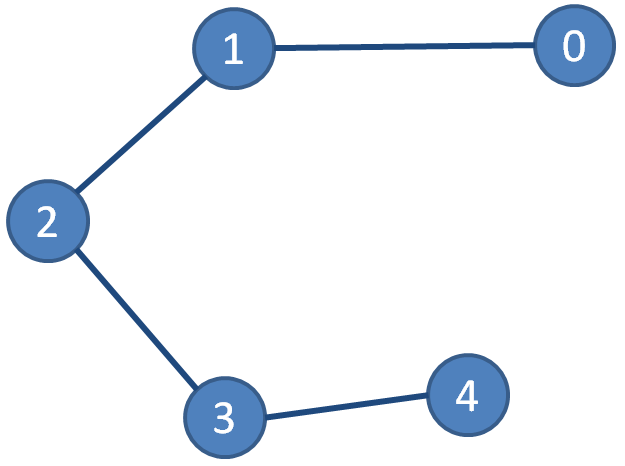
\includegraphics[width=0.8\linewidth]{img/graphe2_1}}{}
\end{minipage}
}}

{\frame{
\frametitle{Chaîne fermée complexe}

\begin{itemize}
 \item Un mécanisme est dit à chaîne fermée complexe, s'il existe des cycles ayant un ou plusieurs arcs communs.
\end{itemize}

\vfill

\begin{minipage}{0.48\linewidth}
 \centering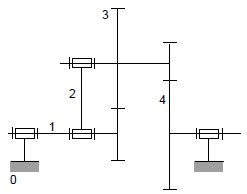
\includegraphics[width=0.8\linewidth]{img/graphe3}
\end{minipage}
\hfill
\begin{minipage}{0.48\linewidth}
\ifdef{\public}{\centering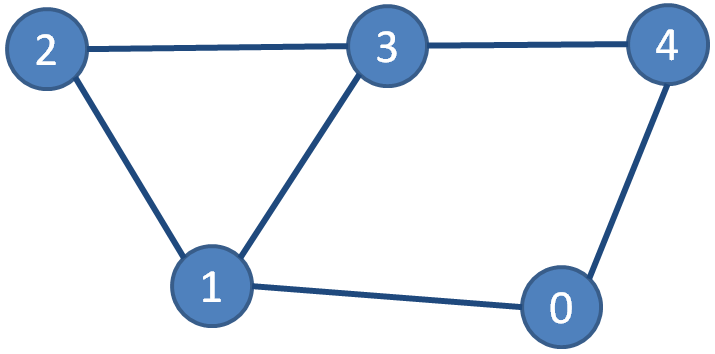
\includegraphics[width=0.8\linewidth]{img/graphe3_1}}{}
\end{minipage}
}}

{\frame{
\frametitle{Théorie des graphes}

\begin{itemize}
 \item La théorie des graphes montre que le nombre de cycles indépendants d'une chaîne fermée complexe se calcule par la relation : $\gamma=l-n+1$,
 \item Dans laquelle :
 \begin{itemize}
	 \item $\gamma$: nombre de cycles indépendants,
	 \item $l$: nombre de liaisons,
 	 \item $n$: nombre de solides (y compris le bâti).
 \end{itemize}
 \item Le nombre $\gamma$ permettra de déterminer le degré de mobilité et le degré d'hyperstatisme d'une chaîne complexe fermée,
 \item Un mécanisme est dit à chaîne fermée complexe, s'il existe des cycles ayant un ou plusieurs arcs communs
 \item \textbf{L'hyperstatisme} apparaît lorsque les pièces subissent plus de contraintes que ce qui est strictement nécessaire pour les maintenir ; au moins un degré de mobilité d'une pièce est supprimé plusieurs fois
\end{itemize}
}}

{\frame{
\frametitle{Liaison équivalente}

La \textbf{liaison équivalente} $le_{1/2}$ à l'ensemble des liaisons situées entre $S_1$ et $S_2$ est une liaison théorique qui aurait le même comportement, c'est à dire transmission de la même action mécanique et autorisation du même mouvement.

\vfill

\begin{minipage}{0.38\linewidth}
 \centering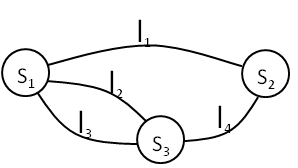
\includegraphics[width=0.6\linewidth]{img/Image1}
\end{minipage}
\begin{minipage}{0.58\linewidth}
Le torseur d'actions mécaniques de la liaison équivalente est noté à $\left\{T_{e(S_1/S_2)}\right\}$.
\end{minipage}

\vfill

\begin{minipage}{0.38\linewidth}
 \centering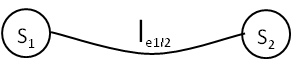
\includegraphics[width=0.6\linewidth]{img/Image2}
\end{minipage}
\begin{minipage}{0.58\linewidth}
Le torseur cinématique de la liaison équivalente est noté $\left\{V_{e(S_1/S_2)}\right\}$.
\end{minipage}
}}

\section{Les liaisons en parallèle}

{\frame{
\frametitle{Liaisons en parallèle}

Des liaisons sont en parallèles si il existe au moins deux liaisons entre deux pièces. 

\vfill

$\left\{T_0\right\}$ représente le torseur des autres \textbf{actions mécaniques extérieures} s'exerçant sur $S_2$.

Le P.F.S. sur $S_2$ avec les $n$ liaisons en parallèles s'écrit:
\begin{math}
  \sum\limits_{i = 1}^n \left\{T_{i(S_2\rightarrow S_1)}\right\}+\left\{T_0\right\}=\left\{0\right\}
\end{math}

Le P.F.S. sur $S_2$ avec la liaison équivalente s'écrit:
\begin{math}
  \left\{T_{e(S_1/S_2)}\right\}+\left\{T_0\right\}=\left\{0\right\}
\end{math}

D'où
\begin{math}
  \left\{T_{e(S_1/S_2)}\right\}=\sum\limits_{i = 1}^n \left\{T_{i(S_2\rightarrow S_1)}\right\}
\end{math}

\vfill

Si un mouvement élémentaire est empêché par une liaison, il est aussi impossible sur les autres liaisons et par suite sur la liaison équivalente.

D'où :

\begin{math}
	\left\{V_{e(S_1/S_2)}\right\}=\left\{V_{1(S_1/S_2)}\right\}=\left\{V_{2(S_1/S_2)}\right\}=...
	=\left\{V_{n(S_1/S_2)}\right\}
\end{math}
}}

{\frame{
\frametitle{Liaisons en parallèle: Exemple de résolution}

\begin{minipage}{0.69\linewidth}
\begin{enumerate}
 \item Chercher le torseur cinématique de la liaison $\left\{V_{e(1/0)}\right\}$.
 \item Chercher le torseur statique de la liaison $\left\{T_{e(1/0)}\right\}$.
 \item Donner le nom de la liaison équivalente.
\end{enumerate}
\end{minipage}
\hfill
\begin{minipage}{0.27\linewidth}
\centering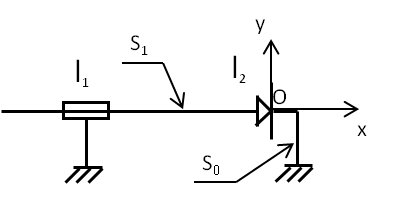
\includegraphics[width=\linewidth]{img/Image3}
\end{minipage}

\vspace{120pt}
}}

{\frame{
\frametitle{Liaisons en parallèle: Hyperstatisme et mobilités}

Le nombre total d'inconnues statiques dans les $n$ liaisons en parallèle est:

\begin{center}
$N_S=\sum\limits_{i = 1}^n n_{si}$
\end{center}

$r$ est le nombre d'équations scalaires indépendantes obtenues par le P.F.S. ($r_s\leq6$).

Le \textbf{degré d'hyperstatisme} $h$ de la liaison équivalente aux $n$ liaisons en parallèle est égal au nombre total $N_S$ d'inconnues statiques moins le nombre $r_S$ de relations indépendantes entre ces inconnues: $h=N_S-r_S$

Le nombre d'équations indépendantes s'écrit alors $r_S=6(p-1)-m$.

Avec:
\begin{itemize}
 \item $p$: nombre de pièces incluant le bâti,
 \item $m$: nombre total de mobilité dans le système.
\end{itemize}
}}

{\frame{
\frametitle{Liaisons en parallèle: Hyperstatisme et mobilités}

Le calcul peut être réalisé avec une étude cinématique.

Ainsi, le nombre total d'inconnues cinématiques dans les $n$ liaisons en parallèle est:

\begin{center}
$I_C=\sum\limits_{i = 1}^n n_{ci}$
\end{center}

Avec $m=I_C-Rg(E)$, $Rg(E)$ étant le rang du système et donc le nombre d'équations indépendantes.

Le degré d'hyperstatisme se calcule ainsi:
\begin{itemize}
 \item $h=E-Rg(E)$ ou,
 \item $h=m-I_C+E$.
\end{itemize}
}}


{\frame{
\frametitle{Liaisons en parallèle: Exemple de résolution}

\begin{minipage}{0.74\linewidth}
\begin{enumerate}
 \item Déterminer le torseur d'actions mécaniques de la liaison. En déduire le nom de cette liaison.
 \item Déterminer le degré hyperstatisme et de mobilité de la liaison.
 \item Localiser les inconnues hyperstatiques. En déduire les contraintes géométriques de position relative des deux liaisons.
\end{enumerate}
\end{minipage}
\hfill
\begin{minipage}{0.22\linewidth}
\centering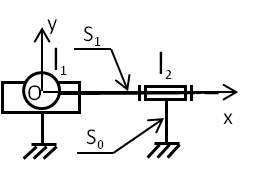
\includegraphics[width=\linewidth]{img/Image4}
\end{minipage}

\vspace{120pt}
}}

\section{Les liaisons en série}

{\frame{
\frametitle{Liaisons en série}
$n$ liaisons sont en série entre deux solides $S_0$ et $S_n$, si elles sont disposées à la suite l'une de l'autre par l'intermédiaire de $(n-1)$ solides. Le solide $S_i$ ($i$ variant de $1$ à $n-1$) n'est soumis qu'à l'action mécanique des solides $S_{i-1}$ et $S_{i+1}$.

\begin{center}
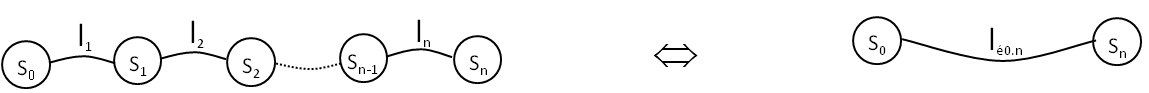
\includegraphics[width=\linewidth]{img/Image5}
\end{center}

Il s'agit d'une chaîne ouverte.
}}

{\frame{
\frametitle{Liaisons en série}

Des liaisons sont en série s'il n'existe qu'un seul chemin entre deux pièces. 

$\left\{T_0\right\}$: torseur des autres \textbf{actions mécaniques extérieures} s'exerçant sur $S_2$.

$\left\{T_i\right\}$: torseur d'actions mécaniques de la liaison $l_i$ (action mécanique de $S_{i-1}$ sur $S_i$).

\begin{itemize}
 \item PFS à $S_0$: $\left\{T_0\right\}-\left\{T_1\right\}=\left\{0\right\}\rightarrow\left\{T_0\right\}=\left\{T_1\right\}$
 \item PFS à $S_0$ et $S_1$: $\left\{T_0\right\}-\left\{T_2\right\}=\left\{0\right\}\rightarrow\left\{T_0\right\}=\left\{T_2\right\}$
 \item PFS à $S_0$,...,$S_n$: $\left\{T_0\right\}-\left\{T_n\right\}=\left\{0\right\}\rightarrow\left\{T_0\right\}=\left\{T_n\right\}$ soit, $\left\{T_{e(0.n)}\right\}=\left\{T_{1}\right\}=\left\{T_{2}\right\}=...=\left\{T_{n}\right\}$
\end{itemize}

\vfill

$\left\{V_{i(S_i\rightarrow S_{i-1})}\right\}$: torseur cinématique de la liaison $l_i$ de $S_i$ par rapport à $S_{i-1}$.

$\left\{V_{e(S_n/S_0)}\right\}$: torseur cinématique de la liaison équivalente $le_{0/n}$ de $S_n$ par rapport à $S_0$


En utilisant la composition des torseurs cinématiques, on écrit :

\begin{math}
	\left\{V_{S_n/S_0}\right\}=\left\{V_{S_n/S_{n-1}}\right\}+\left\{V_{S_{n-1}/S_{n-2}}\right\}+...
	+\left\{V_{S_1/S_0}\right\}
\end{math}, soit $\left\{V_{e(S_n/S_0)}\right\}=\sum\limits_{i = 1}^n \left\{V_i\right\}$

}}


{\frame{
\frametitle{Liaisons en série: Hyperstatisme et mobilité}

\textbf{Hyperstatisme}

La relation précédente permet de calculer toutes les composantes des torseurs d'actions mécaniques $\left\{T_i\right\}$ en fonction de celle de $\left\{T_{e(0/n)}\right\}$

D'où la liaison équivalente $le_{0/n}$ est toujours isostatique : $h=0$.

\textbf{Mobilité}

Le \textbf{degré de mobilité} $m_u$ de la liaison équivalente est égal au nombre d'inconnues cinématiques indépendantes du torseur cinématique de la liaison équivalente.

$m_u$ est aussi le degré de mobilité utile de la chaîne continue ouverte, soit $N_C=\sum\limits_{i = 1}^n n_{Ci}$

Aucun mouvement élémentaire de la liaison $l_i$ est interdit par une autre liaison entre $S_0$ et $S_n$, donc le degré de mobilité $m$ de la chaîne continue ouverte est égal à $N_C$.

On pose :  $m=m_u+m_i$, $m_i$ est le degré de mobilité interne de la chaîne continue ouverte.

Exemple : rotation sur lui même de l'axe d'un vérin.
}}

{\frame{
\frametitle{Liaisons en série: Exemple}

\begin{minipage}{0.74\linewidth}
\begin{enumerate}
 \item Déterminer le torseur statique de la liaison entre $S_0$ et $S_2$.
 \item Déterminer le torseur cinématique de la liaison entre $S_0$ et $S_2$. Quel est le nom de cette liaison équivalente.
 \item Déterminer $m_i$.
\end{enumerate}
\end{minipage}
\hfill
\begin{minipage}{0.22\linewidth}
\centering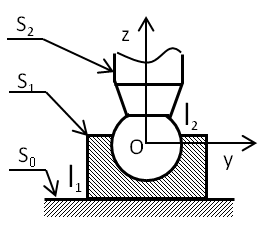
\includegraphics[width=\linewidth]{img/Image6}
\end{minipage}

\vspace{150pt}
}}

{\frame{
\frametitle{Théorie des mécanismes}

\begin{savoir}
\begin{itemize}
 \item Vous devez être capables de modéliser et de résoudre n'importe quel problème de cinématique,
 \item La modélisation des problèmes hyperstatiques doit être effectuée en prenant des précautions.
\end{itemize}
\end{savoir}

\vfill

\begin{obj}
 \begin{itemize}
  \item Déterminer les lois d'entrée/sortie de mécanismes à partir de la fermeture de chaînes mécaniques.
 \end{itemize}
\end{obj}

}}



\end{document}